\documentclass{article}

\usepackage{cite}
\usepackage{graphicx}
\usepackage{wrapfig}

\title{Final Project Literature Review}
\author{Christian Ulfert}
\date{\today}

\begin{document}

\maketitle

\tableofcontents    

\section{Existing work}
\subsection{Tetris}
\paragraph{Introduction}
Tetris is one of the most popular games in the history of computer gaming. Developed in 1984 by Alexey Pajitnov, as a testbed for emerging computing hardware it has trancended its initial purpose and become a cultural icon. 
After initial struggles to leave the UDSSR the big break came when Nintendo bundled it with the original Gameboy in 1989. 
Through capturing a whole generation of newly computer-affine people it has cemented its place in gaming history. The total estimated sales of Tetris are over 500 million copies, most of them in digital form, which only came reality 3 decades after the inital game was developed.
It has also captured the imagination of countless scientists and mathematicians, who have studied the game from a variety of perspectives (computer science, psychology, medicine, mathematics...).
\paragraph{Gameplay}
The staple of tetris is the tetrominoe. A collection of 4 squares arranged in different shapes. The tetrominoes fall from the top of the screen into a 10x20 playing field, they can not be stopped. The player rotates and moves these shapes to arrange them at the bottom of the playing field in a way such they cover a whole row. A full row will be removed from the playing field, giving the player more room to place blocks, and changing the arrangement of the blocks, potentially opening new positions for the next blocks.
In addition the player receives a score for each row removed. The score is higher for removing multiple rows at once. The game ends when the playing field is full and no more blocks can be placed.
\begin{figure}
    \label{fig:poly}
    \centering
    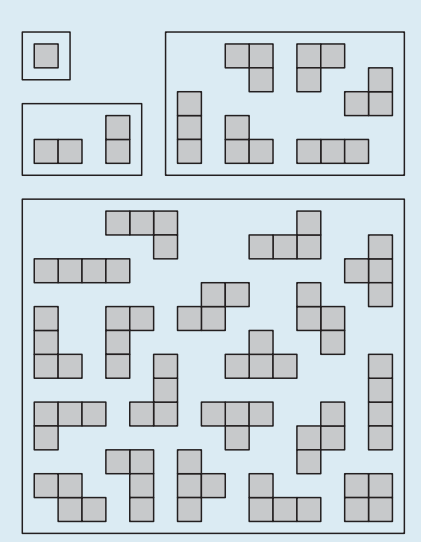
\includegraphics[width=0.6\textwidth]{polynominoes.png}
    \caption{The single monomino (A(1) = 1),
    the two dominoes (A(2) = 2), the A(3) = 6
    triominoes, and the A(4) = 19 tetrominoes
    (Tetris pieces) \cite{polyominoes}}  
\end{figure}
Tetrominoes are a special case of polyominoes (A(4)), which are shapes made up of squares. This is another interesting field of study, and a possible route to increase complexity in tetris, as the number of possible shapes increases dramatically as discussed in Barequet et al.\cite{polyominoes} and visualized in Figure \ref{fig:poly}.
This path however will not be followed in this project.
\paragraph{Mathematics}
There are few computer games whose mathematical properties have been research to the same degree as Tetrises. The following section will give a short but incomplete overview.
\subparagraph*{Tiling} is a funamental problem in mathematics. It deals with the problem of covering a plane with a set of geometric shapes. While this relates directly to the gamesplay, it has also found interes in scientific research such as robotics \cite{tiling1} or neuroscience \cite{tiling2}. While these articles do not require the existence of Tetris, it has certainly sparked intereset in the domain and helped with visualiing and understanding the problem.
\subparagraph*{Complexity - } One of the most renowned scientific papers in game-related computer science is a proof by Demaine et al. that Tetris is NP-complete \cite{tetris_np}. 
Beeing NP-complete means that Tetris is at least as hard as the hardest problems in NP, which are the problems that can be solved in polynomial time by a non-deterministic Turing machine. This means Tetris is one of the hardest problems in computer science.
\newline
\newline
While all this does not influence the development of our 4D Tetris variant, it does inspire how far such a simple game can grow. And there is a hope that a variant in a more complex space will intice similar research.

\paragraph{User Interface}
Part of the success of Tetris is its accessability. There is no need to explain anything. The main menu features a button named "Start" and the game is controlled. The game screen shows the playing field and the rest of the screen is used to display the next block, the score, the level and the lines cleared. 
There is no explanation needed. This is a feature that needs to be replicated to make the game accessible to a broad audience. The difficulty will be to translate the increased compelxity of this project into an accessable product.
\paragraph{Conclusion}
Tetris was a pivotal work. There is a reason it is displayed in the Museum of Modern Art in New York. It has inspired so many different fields and captured millions of players. This all needs to be kept in mind during developemtn as I want to capture a similar feeling of simplicity and complexity in our game.


\subsection{Frac 4D}
This is a game developed in the early 90's and never completed. It featured 4 distinct, but connected 3 dimensional playing fields. Pieces can be rotated and due to their underlying 4 dimensional structure this will reveal different configurations, the can exist in some of the fields but not in others, which can lead to unexpected 'collisions'. The game was apparently very hard to play and in the end failed to provide an easy access into 4 dimenesion.
\begin{figure}
    \label{fig:frac4d}
    \centering
    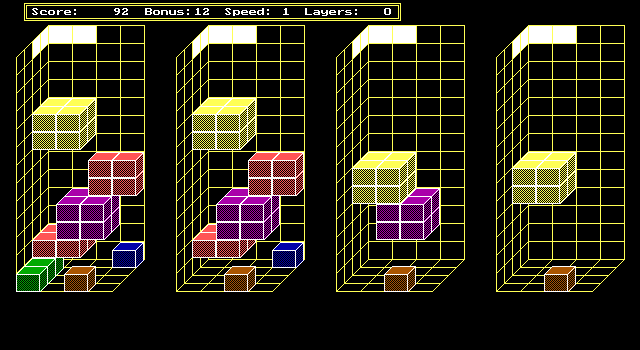
\includegraphics[width=0.6\textwidth]{frac4d.png}
    \caption{The 4 playing fields of Frac 4D. Image from myabandonware.com}
\end{figure}

\subparagraph*{Conclusion}
This game was probably the first 4D adaption of Tetris, and while featuring interesting concepts failed to succeed. There is however features that can be taken from this attempt, especially the highlighting of the corresponding position in the playing field to help the player as seen in Figure \ref{fig:frac4d}.
\subsection{4DTris}
This was another venture into the 4th dimension with Tetris. The concept however is completely different. This time the actual playing field exists in 4 dimensions and the pieces do as well. The playing field is projected into a hypercube, as are the pieces, which ends up looking at a cube the is beeing filled from the inside with different cubes. Development was stopped in 2012 and the author moved on, eventually trying to revive it in 2018, failing. The concept is very interesting, but very hard to imagine. While playing the game might make on proficient, the learning curve would be to steep for most.
\subparagraph*{Conclusion}
For me this is an example of a variant that went to far. While very intersting in concept, the sheer complexity of the gameplay automatically limits the addressable market. In this project falling into the same trap needs to be avoided by creating something fun for many different audiences.
\begin{figure}
    \label{fig:4dtris}
    \centering
    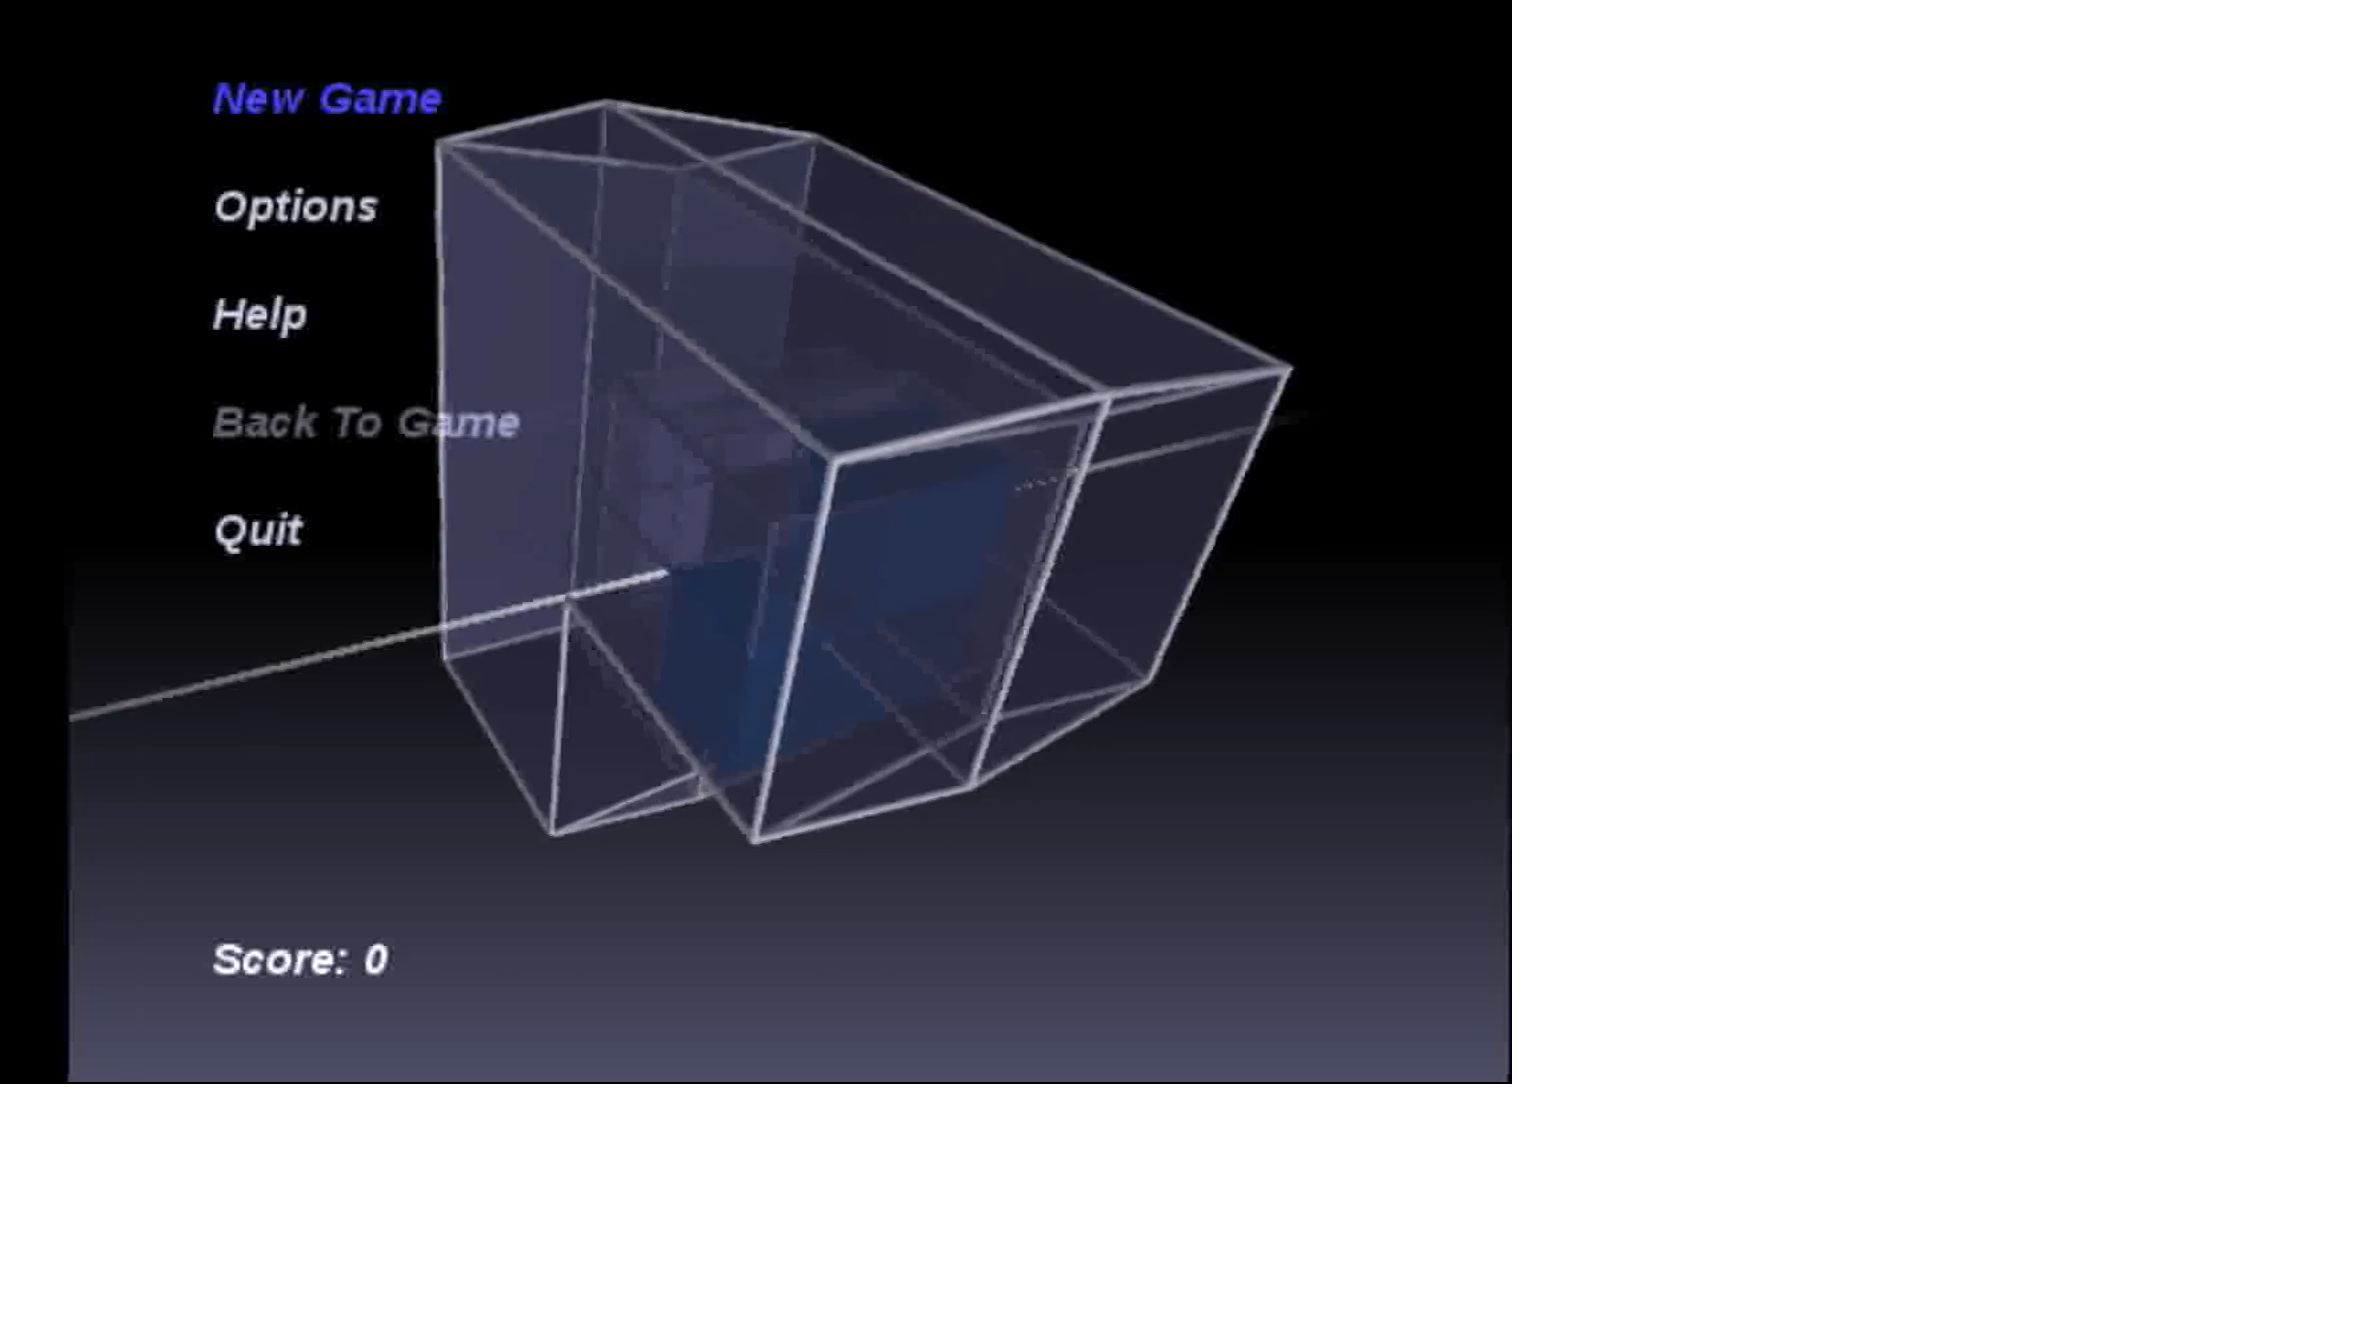
\includegraphics[width=0.6\textwidth]{4dtris.png}
    \caption{4DTris in action. Still from a video on youtube, posted by the autor Simon Laszlo, https://www.youtube.com/watch?v=WO9SNW5Tp7A}
\end{figure}
\subsection{BlockOut}
BlockOut is a 3D Tetris variant. The playing field is a 3D cube and the pieces are 3D shapes. 
The playing field is projected from above. Individual layers are color coded. In any other way the game is very similar to Tetris. The game was moderately successful and can be played online for free nowadays.
\subparagraph*{Conclusion}
This is a great example of a Tetris variant and something that my version will largely be based on. I want to take large parts of the visualization style but enhance on UI/UX.

\subsection{This project}
will be an amalgamation of all the above. Taking the best features from every item. Looks from BlockOut, physics from 4DTris, UX features from Frac4D and general greatness from Tetris.
\section{Literature}
Understanding 4 dimensional space and its implications is a very challenging undertaking, however there is some literature out there that can help with the process. 

\subsection{The Fourth Dimension} by Rudy Rucker \cite{rucker} takes us through a wild journey from ancient mathematics to conteporary philosphy and the other way round. This can create great insights on how it is possible to understnad
and even visualize 4 dimensional object within reality that is confined to 3 dimensions. This work does greatly help with becoming comfortable with the concept of 4 dimensions and will be a great help in the development of the game.
\begin{wrapfigure}{r}{.3\textwidth}
    \label{fig:4d}
    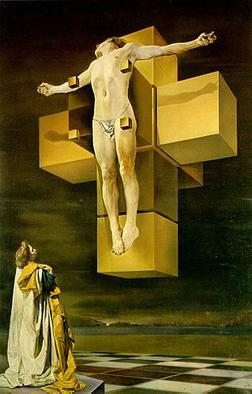
\includegraphics[width=0.6\textwidth]{Dali_Crucifixion_hypercube.jpg}
    \caption{The Crucifixion (Corpus Hypercubus) by Salvador Dali. A representation of a hypercube unfolded into 3 dimensions.}
\end{wrapfigure}
\subsection{Geometric algebra for computer science} by Leo Dorst, Daniel Fontijne and Stephen Mann \cite{geo_alg} serves as a great introduction into geometric algebra, which might be a solution to the problem of representing, and especially rotation 4 dimensional ojects. While no final decision has been made on the technique that will be used, a decent understanding of the topice is necessery to finally choose the correct one. 
\subsection{An Introduction to Clifford Algebras and Spinors} by Jayme Vaz Jr. and Roldao da Rocha Jr. \cite{cliff_alg} is another great resource into the topic, especially as Cliffor algebras are widely used in n-dimensional geometry. The chapter on spinors is especially interesting as they are one of the ways to represent rotations in higher dimensions and might be the foundation of the techniques we will use.
\subsection{On Rotations in Space of Four Dimensions} by Cole \cite{rot_n_1} is an article from 1888 that deals with the problem of rotations in 4 dimensions. The article proofs a general rotation matrix for 4 dimensions. The most important feature however is the date of publication, prooving the persistant human interest in the topic of higher dimensions and therefore (somewhat) validating the project.
\subsection{Conclusion}
This is just a small outtake on literature that can help understand the topic of higher dimensions which is necessary for this project. Especially the decision on which mathematical representation and technique will be chosen is heavily informed by these books/articles.
\section{Visualization}

Visualization of 4 dimensional objects is a very challenging but interesting task.

There is a large amount of great resources available to help understanding how this can be done. A very good overview over the techniques is presented in the PhD thesis by Hallasch \cite{4d_vis_1}. In extension to this the website "https://baileysnyder.com/interactive-4d/4d-cubes/" \cite{4d_vis_2} offers great interactive tools to generate an understanding of how to get to 4d dimensions and back.
\subsection{Illuminating the fourth dimension} by Hanson et al. \cite{4d_vis_3} describes multiple techniques on how to render 4d objects into 3d space onto a 2d screen. This includes advanced shadowing and shading techniques which exceed the necessitiy of this project since unity will be used.


\bibliographystyle{acm}
\bibliography{references}

\end{document}